\documentclass[../main/main.tex]{subfiles}
\begin{document}

% \dominitoc
% \faketableofcontents
% \dominilof
% \fakelistoffigures
% \dominilot
% \fakelistoftables

\chapter{Cr\'eation d'un \'echantillon complet}\label{ch:sample}
\epigraph{\openquote La scène disparaît et devient l'un des
acteurs.\closequote}{Robin \textsc{Gaillard}}

Nous avons vu Chapitre~\ref{ch:cosmo} que l'amélioration des mesures de
paramètres cosmologiques par le diagramme de \textsc{Hubble} nécessite une
meilleure précision dans la connaissance astrophysique des SNe~Ia, afin,
notamment, de permettre la réduction des incertitudes systématiques. À cet
effet, une évolution des propriétés intrinsèques des SNe~Ia inconnue fausserait
ces résultats.

Nous avons vu Chapitre~\ref{ch:env} que l'environnement des supernovae avait un
impact non négligeable sur leurs caractéristiques mesurées, et notamment leur
appartenance à la sous-population «~jeune~» ou «~vieille~». Dans la perspective
de mesurer une évolution de la luminosité intrinsèque des SNe~Ia, notre
recherche se base sur le modèle d'évolution de l'âge moyen de \cite{rigault2020}
des SNe~Ia et étudie les variations de leur étirement en fonction de l'âge (voir
Chapitre~\ref{ch:stretch}).

Nous présentons dans ce chapitre l'échantillon sur lequel nous effectuons ces
mesures. Nous discutons dans un premier temps des qualités qu'un tel échantillon
doit présenter Section~\ref{sec:compl}, avant de le réaliser et de le présenter
Section~\ref{sec:sample}. La Section~\ref{sec:ztfsam} en présente l'augmentation
\textit{via} l'implémentation des données de ZTF aux sondages.

\vfill
\minitoc
\vfill
\newpage

\section{Notion de complétude}\label{sec:compl}

% \textsc{Malmquist} bias :~\cite{perrett2010}

Cette thèse repose sur l'étude statistique des propriétés des SNe~Ia, et donc en
premier lieu sur l'échantillon de données sur lesquelles développer notre
raisonnement. Pour qu'il soit intéressant il doit être suffisamment grand, mais
également représentatif de la population des SNe~Ia. En effet, nous avons vu
Chapitre~\ref{ch:env} que les SNe~Ia sont corrélées avec leur environnement.
Comme nous souhaitons étudier toute la zoologie des SNe~Ia et non pas une
catégorie particulière (par exemple, celles se trouvant uniquement dans des
galaxies de masse $M_* > \SI{10}{\Msun}$), nous nous intéressons à des données
ne comportant pas de biais de la sorte. De même, nous avons vu que pour être de
qualité cosmologique, leurs caractéristiques d'étirement et de couleur sont
respectivement comprises entre $\pm3$ et $\pm0,3$. Pour que cet échantillon soit
représentatif de la population des SNe~Ia, nous voulons que les données le
constituant se rapprochent le plus possible d'un tirage aléatoire de toutes les
SNe~Ia dans la nature, et non pas, par exemple, d'une seule sous-partie
uniquement composée de SNe d'étirement entre $\pm2$. Nous définissons alors cet
échantillon comme «~complet~». Ce concept est largement dépendant de la manière
dont les données sont relevées.

\subsection{Stratégies d'observation}\label{ssec:stratobs}

Les supernovae sont des phénomènes transitoires, c'est-à-dire des objets dont le
flux lumineux varie dans le temps, et elles sont également brèves et rares~:
elles durent typiquement quelques semaines et surviennent environ une fois par
siècle et par galaxie. Leur observation requiert donc des stratégies
particulières. Pour déterminer leurs courbes de lumière (\ref{ssec:lc}), il est
nécessaire d'avoir un champ de mesure suffisamment profond pour ne pas se
contenter que de leur luminosité au maximum. Différentes approches peuvent
entrer en jeu~: les recherches ciblées et les recherches non-ciblées.

\paragraph*{Les recherches ciblées} consistent à se focaliser sur des amas de
galaxies connus en vue d'augmenter la probabilité d'observer des supernovae. Il
paraît en effet évident que plus la concentration en étoiles est forte, plus
nous nous attendons à une haute probabilité que certaines d'entre elles
entament leur fin de vie et leur explosion en supernovae. Cependant, une telle
pratique implique une sélection des environnements des SNe et donc un biais sur
la nature des données recueillies. Dans le cas des amas de galaxies,
l'environnement favorisé sera celui contenant des progéniteurs vieux, dans des
galaxies massives avec peu de formation stellaire. Afin d'étudier la potentielle
évolution de la population des SNe, il faut réduire au maximum ces biais et
favoriser la récolte d'un échantillon représentatif de toute la zoologie des
SNe~Ia.

\paragraph*{Les recherches non-ciblées} utilisent de grands champs de caméra pour
sonder de larges portions du ciel. Originellement
\citep[SCP,][]{perlmutter1999}, leur procédé était d'effectuer une
détection photométrique avant d'opérer une identification spectroscopique,
confirmant leur caractère de SN~Ia ou non, pour finalement décider de programmer
ou non un suivi photométrique permettant l'établissement de leur courbe de
lumière. Une telle pratique limite les biais mais donne des courbes de lumières
pauvres en points de mesure avant le maximum de luminosité, impactant
l'ajustement des courbes. Ces méthodes ont évolué pour devenir des recherches
\textit{glissantes} \citep{astier2006}. Elles consistent à balayer régulièrement
le ciel en observant un même champ dans un même filtre de manière répétée tous
les quelques jours, afin d'à la fois détecter et extraire les courbes de
lumières des SNe~Ia, même si leur identification est effectuée après leur
maximum de luminosité.

\subsection{Biais de \textsc{Malmquist} et solution}\label{ssec:malm}

De tels sondages ne sont cependant pas exempts d'effets de sélection. En effet,
même une recherche glissante s'effectue avec un appareil de mesure ayant une
capacité limitée à détecter une source lumineuse~: les objets de magnitude
apparente plus élevée (luminosité plus faible) que ce seuil de détection ne
seront pas inclus. De tels sondages sont dits à magnitude limitée. Or, comme
chaque astre voit sa luminosité décroître avec le carré de la distance qui le
sépare de l'observation (\ref{ssec:dl}), cette limite implique que les astres de
magnitude absolue plus élevée seront relevés à de plus grandes distances que les
autres, laissant croire qu'à partir d'une certaine distance les objets sont
intrinsèquement plus lumineux.

Dans le cadre des SNe~Ia dont nous supposons la magnitude absolue similaire,
nous pourrions en première approche négliger cet effet. Cependant, comme exposé
en Section~\ref{ssec:corr}, il a été déterminé que la magnitude absolue des
supernovae de type Ia est corrélée avec leur étirement et leur couleur, de telle
sorte que les plus faibles soient celles de petit étirement et de couleur rouge.
Ainsi, proche du seuil de détection, les SNe~Ia ne sont pas sélectionnées de
manière homogène, et l'échantillon recueilli sera une sous-population laissant
penser qu'avec la distance, les SNe~Ia ont en moyenne un plus haut étirement et
sont de couleur bleue.

Le cadre de notre étude nécessite un échantillon que nous appelons
«~volume-limité~», pour lequel nous supposons que la population résulte bien
d'un tirage aléatoire de ce qui existe dans la nature. Les sondages modernes
reposant sur des recherches glissantes, il nous a fallu les réduire pour les
utiliser.

\section{Échantillon d'étude}\label{sec:sample}

Nous détaillons dans cette Section la procédure de construction de notre
échantillon volume-limité comme expliqué partie~\ref{ssec:malm}. Notre étude se
base sur les données de la combinaison de sondages Pantheon \citep{scolnic2018},
en remplaçant la combinaison ciblée LOWZ par les données SNfactory dont la
sélection est maîtrisée et permettant une étude de sous-population grâce au
LsSFR. Les données de HST étant complètes, la confection de notre échantillon se
concentre sur les sondages SDSS, PS1 et SNLS~; leur nature non-ciblée et limitée
en magnitude permet d'en construire une portion limitée en volume comme décrit
Section~\ref{sec:compl}.

\subsection{Confection}\label{ssec:cuts}

Nous détaillons ici deux des approches mises en place visant à déterminer la
portion des sondages que nous pouvons considérer comme étant limitées en volume.

\subsubsection{Approche statistique}\label{sssec:baserate}

À partir des données publiées dans~\cite{scolnic2018}\footnote{\href{
    https://archive.stsci.edu/hlsps/ps1cosmo/scolnic/data_fitres/}
{https://archive.stsci.edu/hlsps/ps1cosmo/scolnic/data\_fitres}}, il est
possible de tracer l'histogramme des SNe~Ia en fonction du redshift (cf.
Sections précédentes, par exemple Figure~\ref{fig:snfhist}, à gauche). En
supposant une densité volumique de supernovae uniforme, chaque intervalle de
redshift comprend un volume de plus en plus grand et nous nous attendons donc à
observer toujours plus de SNe~Ia avec la distance. Nous observons cependant une
baisse de ce nombre à partir d'un certain redshift. La chute du nombre de SNe~Ia
provient de cette limitation du sondage à mesurer la luminosité. Notre première
approche a été de se baser sur une étude statistique pour essayer de récupérer
la valeur estimée à partir de laquelle chaque sondage s'écarte d'un modèle
volumétrique. Le protocole est le suivant~:
\begin{itemize}
    \item Les bornes minimales et maximales des données sont augmentées d'une
        faible valeur aléatoire afin d'assurer une variation du centre des
        intervalles. Par exemple, pour SNLS, nous prenons une limite entre 0,06
        et 0,12 à gauche et entre 1,10 et 1,15 à droite~;
    \item Nous choisissons aléatoirement entre 5 et 20 intervalles pour tracer
        l'histogramme~;
    \item Nous initialisons un modèle volumétrique $a\times
        \left(V(z_2)-V(z_1)\right)$ avec $a$ la densité volumique de SNe~Ia,
        paramètre libre du modèle, auquel nous passons comme donnée les bords
        des intervalles~;
    \item Les valeurs du modèle sont comparées aux hauteurs des intervalles de
        l'histogramme, permettant l'ajustement du modèle par une loi de Poisson
        cumulée \citep[voir par exemple][]{syed2015}. Pour un intervalle donné
        de nombre moyen de données $\lambda$, la probabilité qu'il y en ait
        exactement $k$ est, d'après la loi de Poisson~:
        \begin{equation}\label{eq:poisson}
            p(k) = \mathcal{P}(X = k) = \frac{\lambda^k}{k!}e^{-\lambda}
        \end{equation}
        La fonction de répartition, ou de distribution cumulative, est donnée
        par~:
        \begin{equation}\label{eq:pcdf}
            \mathcal{P}(X\leq x) = \sum_{k=0}^{x}p(k) = e^{-\lambda}
            \sum_{k=0}^{x} \frac{\lambda^k}{k!}
        \end{equation}
    \item Nous choisissons aléatoirement un intervalle maximal après lequel
        l'ajustement s'arrête, avec un minimum de 3 intervalles (6 dans les cas
        des Figures de~\ref{fig:zmax_method}), 10 fois pour chaque histogramme~;
    \item Nous sauvons les positions et valeurs de probabilité des intervalles
        ajustées et créons une interpolation linéaire des résultats~;
    \item Ces 5 étapes sont répétées 1000 fois et nous calculons la médiane et
        l'écart type des 10 000 interpolations calculées.
\end{itemize}

\begin{figure}[ht]
    \centering
    \begin{subfigure}[]{.49\linewidth}
        \centering
        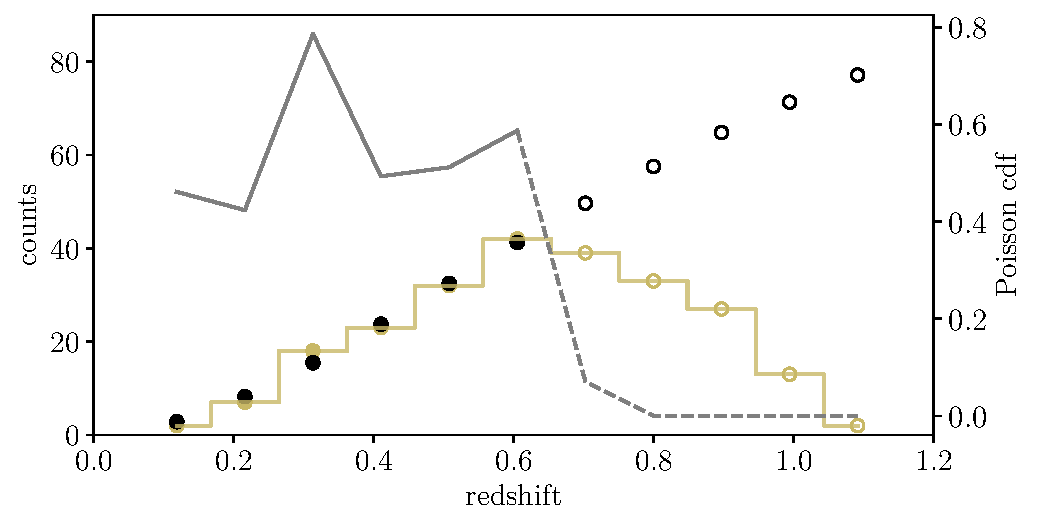
\includegraphics[width=\linewidth]{zmax_method_snls-01}
        \captionsetup{justification=centering}
        \caption{11 intervalles, ajustement sur 6}
        \label{fig:zmax_method1}
    \end{subfigure}
    \begin{subfigure}[]{.49\linewidth}
        \centering
        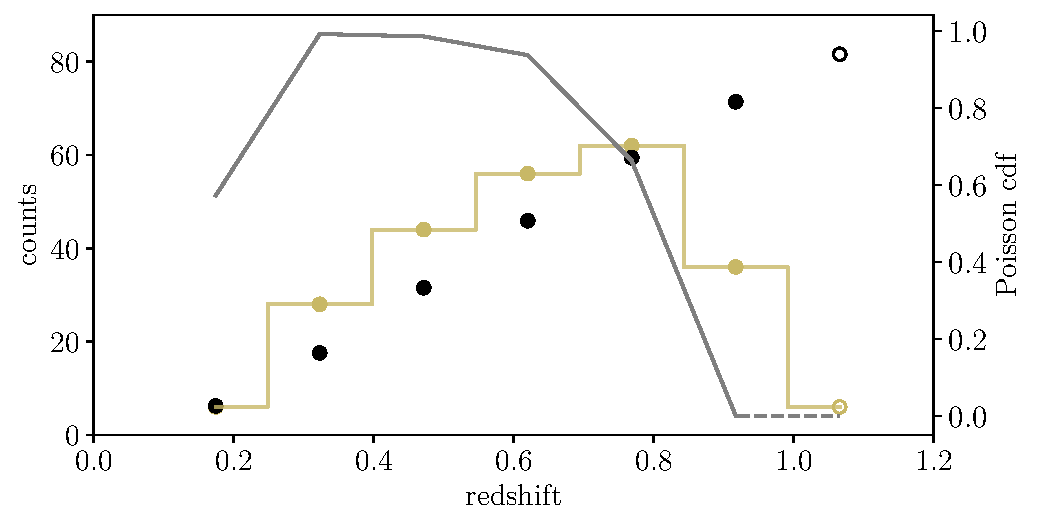
\includegraphics[width=\linewidth]{zmax_method_snls-02}
        \captionsetup{justification=centering}
        \caption{7 intervalles, ajustement sur 6}
        \label{fig:zmax_method2}
    \end{subfigure}
    \captionsetup{justification=centering}
    \caption{Exemple d'ajustement statistique pour deux tirages aléatoires
    d'histogrammes de SNLS.}
    \label{fig:zmax_method}
\end{figure}

% Deux modèles ont été testés. Le premier est issu de \textbf{perrett2012} donnant
% un taux volumétrique co-mobile~:
% \begin{equation}\label{eq:perrett}
%     R(z) = 1.75\times10^{-5}(1+z)^{2,11}\,{\rm yr^{-1}Mpc^{-3}}
% \end{equation}
% Le second est directement issu du calcul d'un volume co-mobile dérivé des
% équations de la relativité générale~:

Le modèle volumétrique retenu dans notre analyse est défini par~:
\begin{equation}\label{eq:comobvol}
    V(z) = \frac{4\pi}{3}\times d_C{}^3(z)
\end{equation}
avec $d_C(z)$ la distance comobile
\begin{align}
    d_C(z)                           & =
    \frac{c}{H_0} \int_{0}^{z} \frac{\d z'}{E(z')}
    \quad\text{avec}\quad\\
    E(z) \triangleq \frac{H(z)}{H_0} & =
    \left[\Omega_R(1+z)^4 + \Omega_M(1+z)^3 +
        \Omega_k(1+z)^2 + \Omega_\Lambda
    \right]^{1/2}
\end{align}

Nous avons choisi la cosmologie issue de la collaboration Planck
\citep{planck2018}, dont les valeurs sont indiquées Table~\ref{tab:planckvals}.

\begin{table}[ht]
    \centering
    \caption[Valeurs des paramètres cosmologiques utilisés pour la détermination
    statistique du redshift limite des sondages SDSS, SNLS et PS1]{Valeurs des
        paramètres cosmologiques utilisés pour la détermination statistique du
    redshift limite des sondages SDSS, SNLS et PS1.}
    \label{tab:planckvals}
    \begin{tabular}{ccccc}
        \toprule
        $H_0$ &
        $\Omega_R$ & $\Omega_M$ & $\Omega_k$ & $\Omega_\Lambda$ \\
        \midrule
        \SI{67,74}{km.Mpc^{-1}.s^{-1}} &
        $5.389\times10^{-5}$ & 0,3075 & 0 & 0,6910 \\ 
        \bottomrule
    \end{tabular}
\end{table}

Le résultat de ces calculs donne une estimation du redshift à partir duquel
chacun des sondages n'a plus la capacité à recueillir toutes les SNe~Ia,
représentée Figure~\ref{fig:zmax_method_results}. En estimant $z_{\lim}$ comme
étant la valeur à laquelle la médiane des distributions cumulées chute à 0,5 et
les erreurs basse et haute à 0,525 et 0,475 respectivement, nous obtenons les
valeurs de la Table~\ref{tab:zlimsample}.

\begin{figure}[ht]
    \centering
    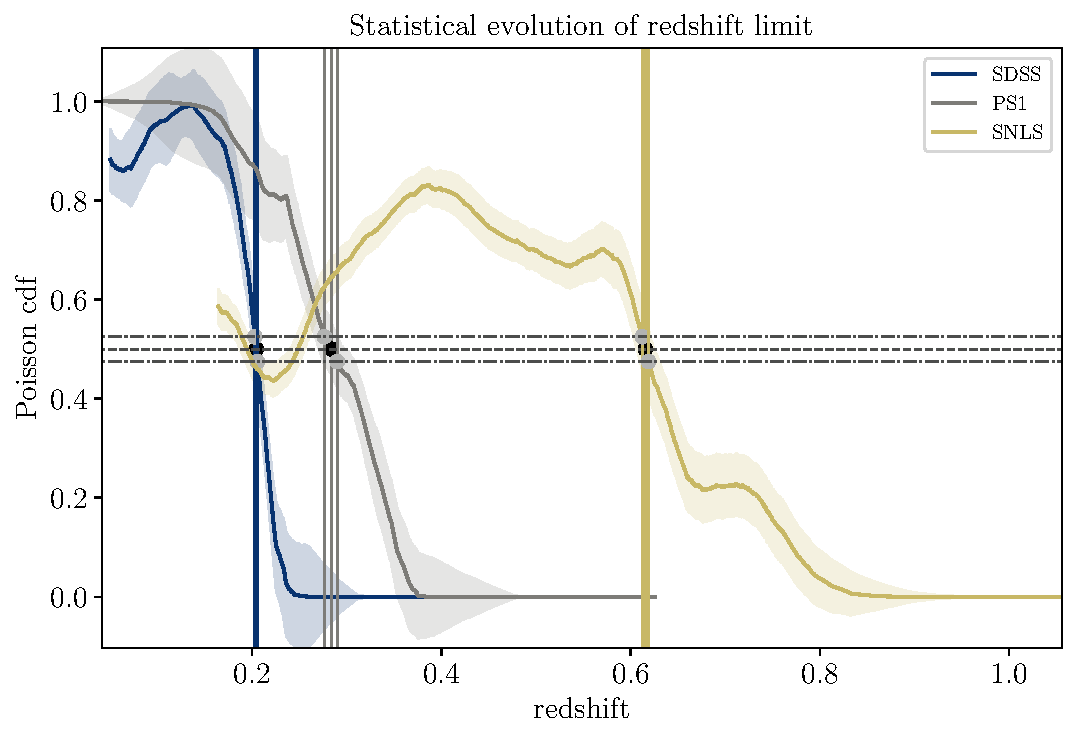
\includegraphics[width=.7\linewidth]{zmax_method_results}
    \captionsetup{justification=centering}
    \caption[Évolution médiane du redshift limite des sondages SDSS, PS1 et SNLS
    par approche statistique]{Résultat graphique de l'évolution médiane de
    l'étude statistique du redshift limite pour les sondages SDSS, PS1, et SNLS}
    \label{fig:zmax_method_results}
\end{figure}

Cette première approche présente une robustesse certaine dans l'établissement
des évolutions statistiques en répétant le processus précédent. Cependant, le
sens de variation non constant du résultat de SNLS et de PS1 ne permet pas
de forte confiance dans la correspondance de ce protocole à l'objectif de cette
étude~; de plus, le choix de la valeur de la fonction de répartition à laquelle
nous pouvons considérer le sondage complet n'est pas motivée mathématiquement ou
physiquement de manière systématique. Cette conclusion nous a amenæ à une
approche combinant à la fois la réalité de la sélection astrophysique
instrumentale et les équations de distribution de luminosité de SN~Ia avec leurs
paramètres $x_1$, $c$ et $z$.

\subsubsection{Approche analytique}\label{sssec:maglim}

En supposant que ces sondages ont un typage spectroscopique et un suivi
photométrique suffisants, ils devraient avoir des effets de sélection de
sous-population de SNe~Ia négligeables en deçà d'un certain redshift permettant
l'acquisition de toute la zoologie d'étirements et de couleurs. Les données de
SNe~Ia issues de l'ajustement par \texttt{SALT2.4} ne contiennent que des
données avec un maximum de $x_1 = \pm 3$ et de $c = \pm 0,3$ \citep[][cf
Section~\ref{ssec:salt}]{guy2007, betoule2014}.

La magnitude absolue d'une supernova à son maximum de luminosité est, d'après
l'équation~\ref{eq:mxc}~:
\begin{equation*}
    M = M_0 -\alpha x_1 + \beta c
\end{equation*}
avec $M_0 = \SI{-19,36}{mag}$ dans le filtre photométrique $B$ de Bessell
\citep{kessler2009a, scolnic2014}, $\alpha=0,158$ et $\beta=3,14$
\citep[Table 7,][]{scolnic2018}. Nous déterminons cette quantité sur l'ellipse
limite des paramètres grâce au paquet \texttt{sncosmo}
\footnote{\href{https://sncosmo.readthedocs.io/en/stable/}
{https://sncosmo.readthedocs.io/en/stable/}}, représentée par un gradient de
couleur Figure~\ref{fig:maglim}. Nous trouvons alors que la supernova la moins
lumineuse est celle de paramètres $x_1 = -1,65$ et $c = 0,25$ dont le maximum de
magnitude absolue standardisée est $M_{\min}^{t_0}=\SI{-18,31}{mag}$.

\begin{figure}
    \centering
    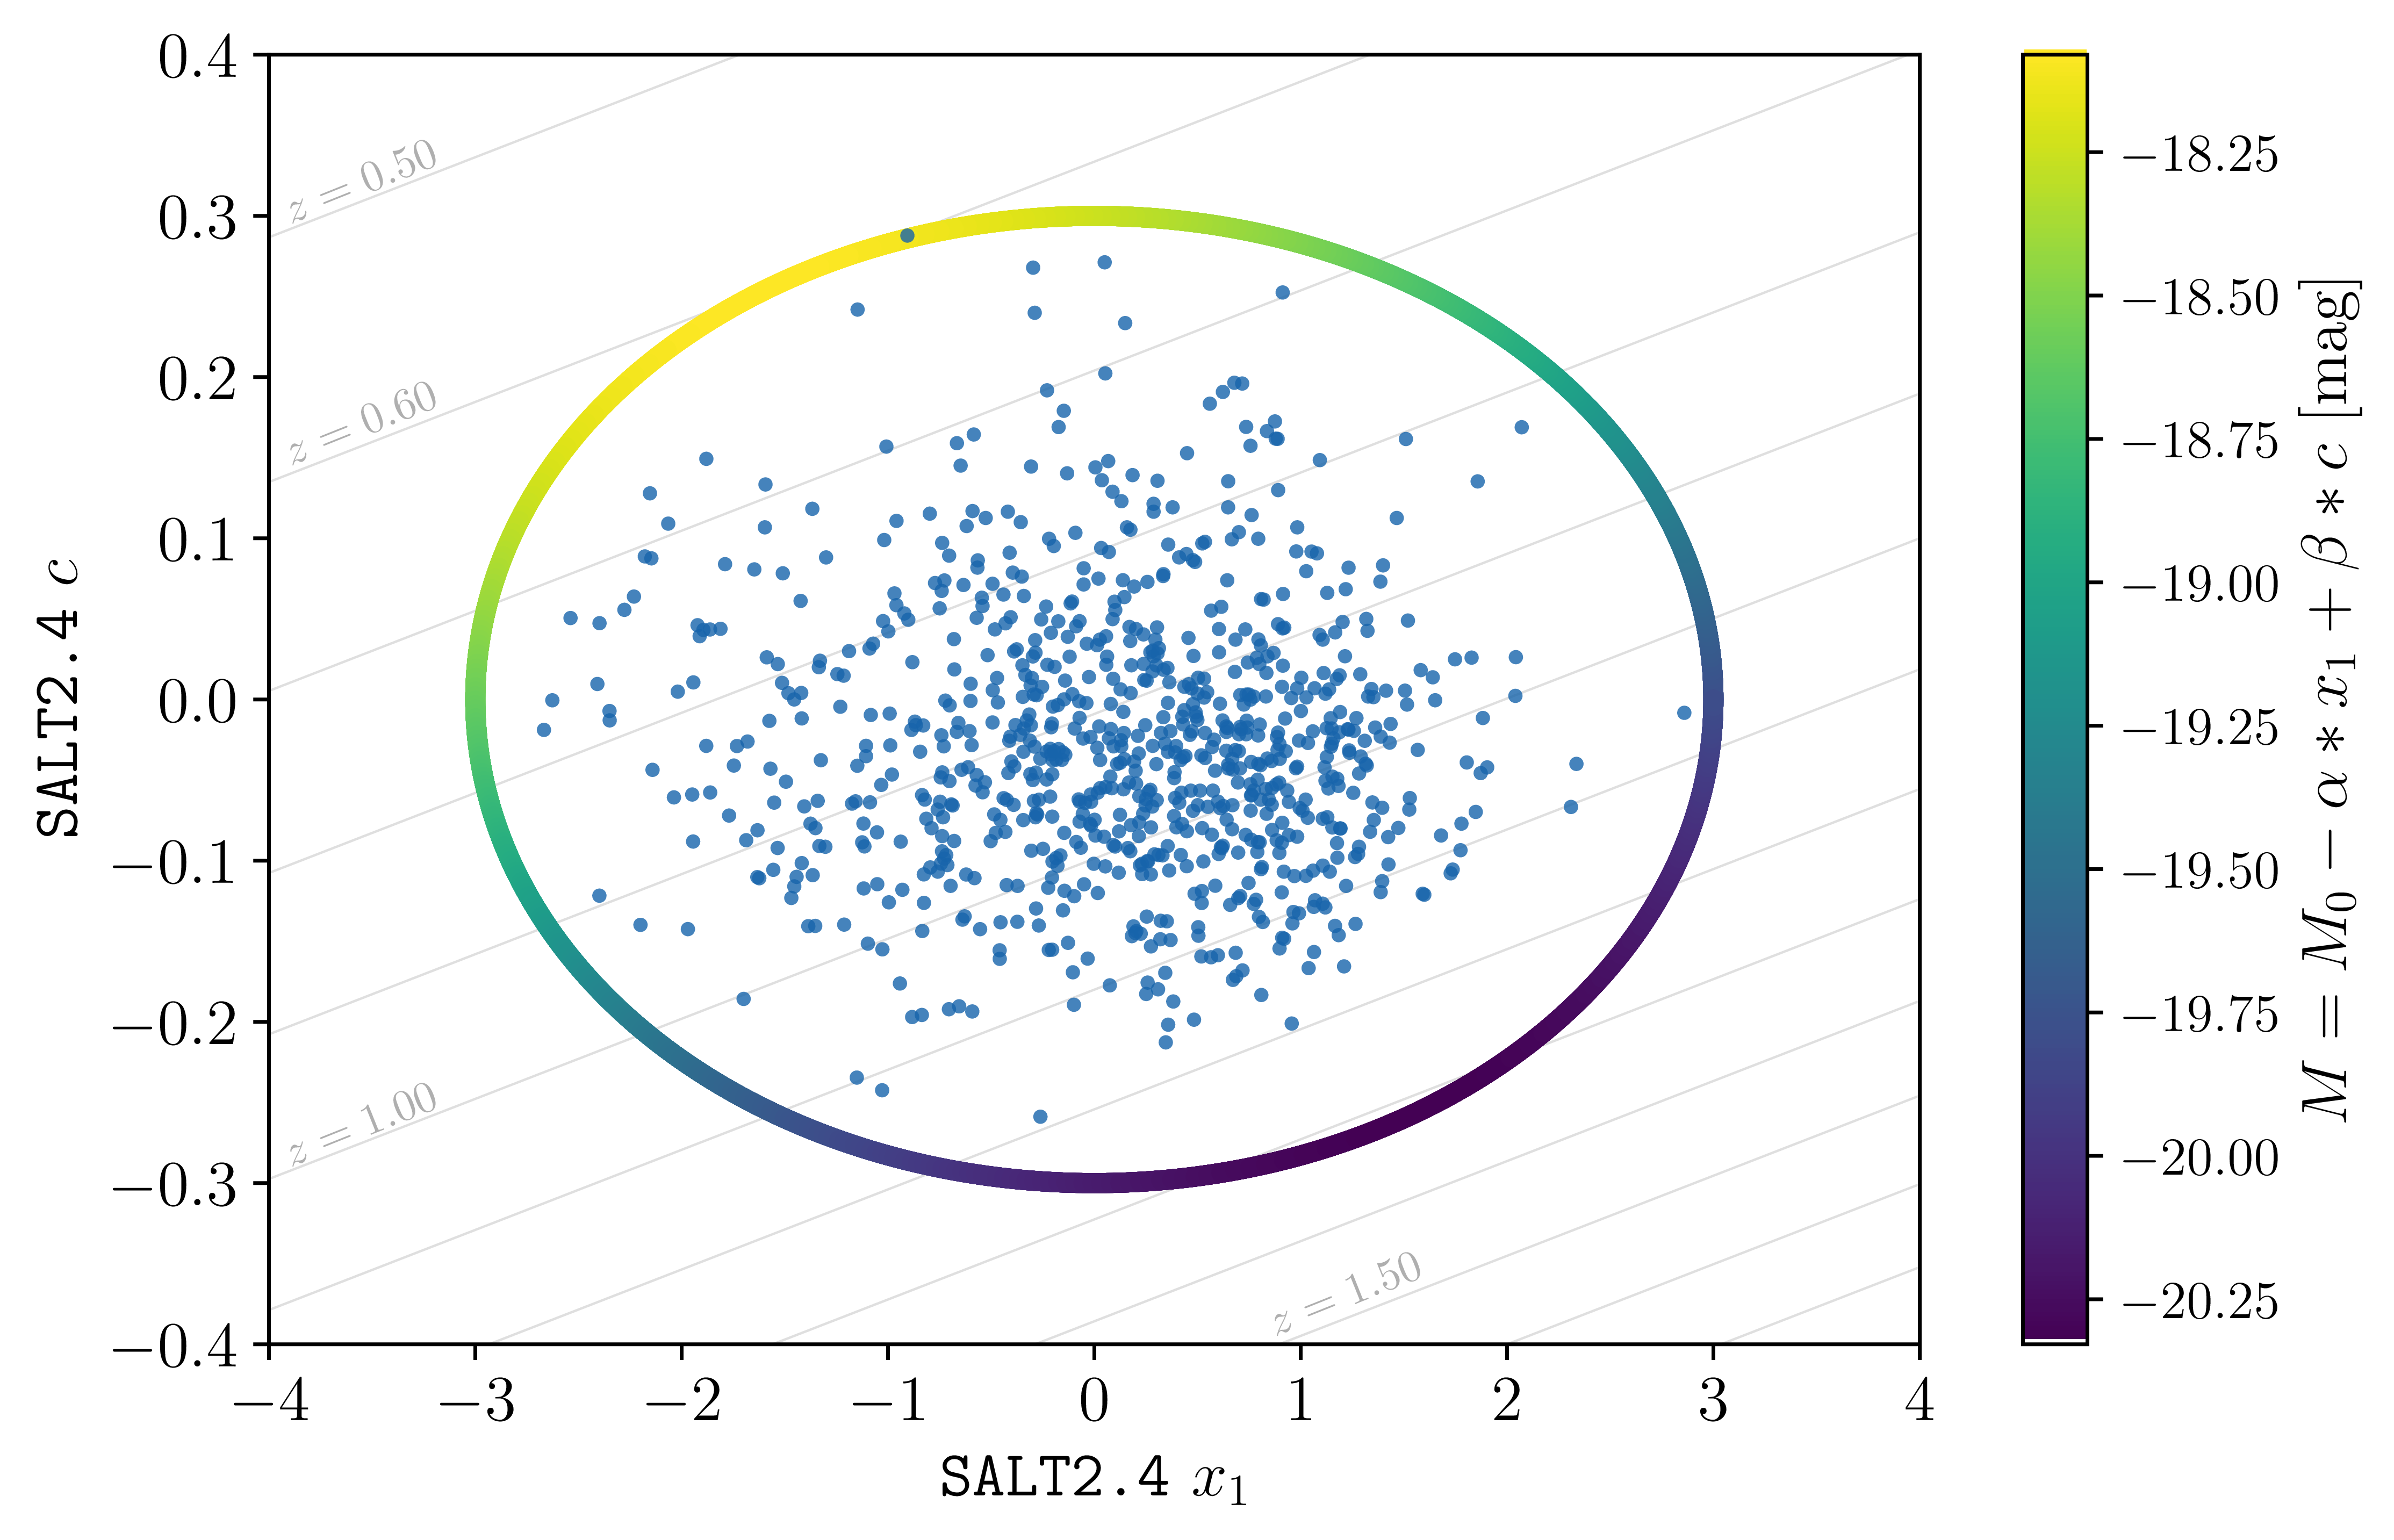
\includegraphics[width=0.95\linewidth]{zmax_maglim_snls}
    \caption[Distribution et limite des paramètres de courbe de lumière
    d'étirement ($x_1$) et de couleur ($c$) des sondages SDSS, PS1 et SNLS
    combinés du catalogue Pantheon]{Distribution des paramètres de courbe de
        lumière d'étirement ($x_1$) et de couleur ($c$) issus d'un ajustement
        par \texttt{SALT2.4} pour les données de SNe~Ia des sondages SDSS, PS1 et
        SNLS combinés du catalogue Pantheon. Chaque supernova est représentée par un
        point bleu. L'ellipse limite des paramètres $(x_1=\pm3, c=\pm0,3)$ est
        représentée avec un gradient de couleur correspondant à la magnitude
        absolue standardisée en utilisant les valeurs de~\cite{scolnic2018} pour
        les coefficients $\alpha$ et $\beta$. Les lignes diagonales grises
        représentent l'évolution de $m = m_{\lim}$ en fonction de $z$ dans le
        plan $(x_1,c)$ entre $z=0,50$ et $z=1,70$ pour la magnitude limite
    $m_{\lim}=\SI{24,8}{mag}$ du sondage SNLS.}
    \label{fig:maglim}
\end{figure}

Cependant, pour établir une courbe de lumière, une supernova doit être observée
typiquement au moins 5 jours avant et 1 semaine après son pic de luminosité,
donnant une magnitude absolue limite effective d'approximativement $M_{\lim} =
\SI{-18,00}{mag}$. En connaissant les magnitudes limites de chaque sondage et
avec l'équation reliant le module de distance aux magnitudes observée et absolue
\begin{equation}\label{eq:distmod}
    \mu(z) = m - M
\end{equation}
nous pouvons déterminer le redshift limite $z_{\lim}$ au-delà duquel la SN~Ia la
moins lumineuse ne sera pas observée. Nous avons ainsi défini un ensemble de
redshifts limites définissant un échantillon fiduciel en choisissant la limite
suggérée par cette analyse.

Cependant, cette solution pourrait ne pas être optimale étant donné qu'elle
ignore les efficacités de suivi spectroscopiques pour les redshifts en-dessous
de $z_{\lim}$~; c'est pourquoi nous avons également déterminé un autre ensemble
de coupes définissant un échantillon «~conservatif~». Cet échantillon est plus
petit et donc sera statistiquement moins pertinent, mais également moins sujet
aux effets de sélection. Ainsi, si l'évolution des propriétés des SNe~Ia avec le
redshift est encore sondable dans l'échantillon conservatif, il serait encore
plus présent dans un échantillon dont l'absence d'effets de sélection est
effectuée avec plus de précision que nos coupes en redshift.

Nous présentons Figure~\ref{fig:speceff} les différentes efficacités
spectroscopiques avec le redshift des 4 sondages LOWZ, SDSS, PS1 et SNLS. Nous y
observons que les magnitudes limites correspondent également aux limites des
capacités spectroscopiques, mais ces seuls critères ne suffisent pas à rendre
compte de la qualité limitée en volume d'un sondage. Nous détaillons maintenant
les choix pour les sous-échantillons concernés par ces coupes.

\begin{SCfigure}[1][h!]
    \centering
    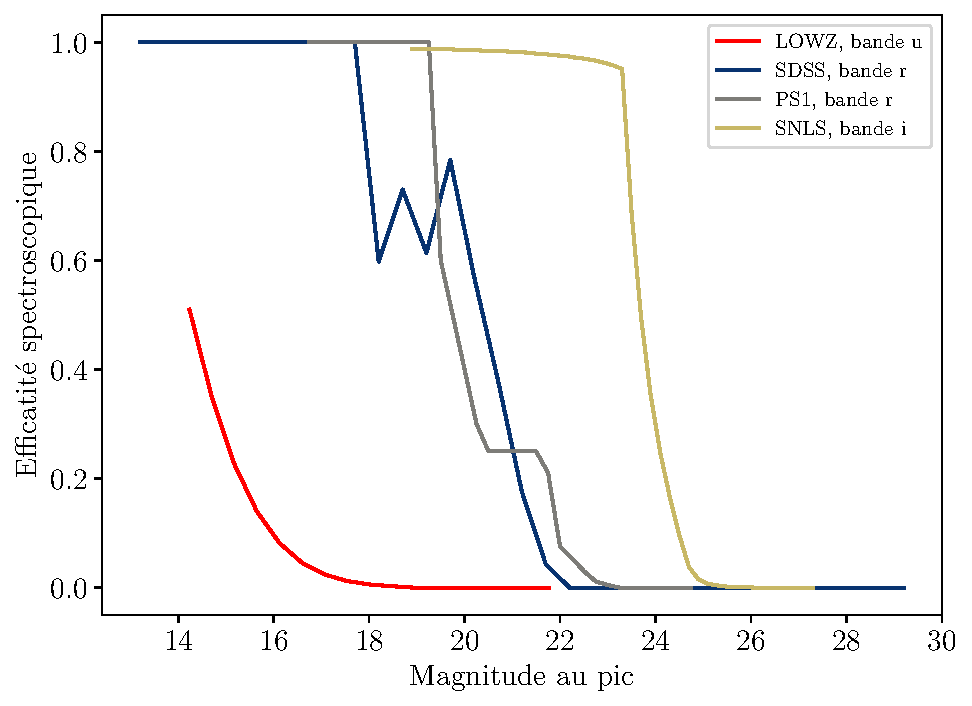
\includegraphics[width=.5\linewidth]{speceff-all}
    % \captionsetup{justification=centering}
    \caption[Comparaison des efficacités spectroscopiques des différents
    sondages]{Comparaison des efficacités spectroscopiques des différents
        sondages. Figure produite avec les données de la collaboration
        \textit{Dark Energy Survey} \citep[DES,][]{abbott2019} pour LOWZ, de
        Pantheon \citep{scolnic2018} pour PS1, et de Pantheon+
    \citep{popovic2021b} pour SDSS et SNLS.}
    \label{fig:speceff}
\end{SCfigure}

\paragraph*{Pour SNLS} dont les supernovae sont typiquement entre $0,4 < z <
0,8$, la bande $B$ de Bessell dans un référentiel au repos correspond
approximativement à son filtre $i$, de magnitude limite à 5$\sigma$ de
\SI{24,8}{mag}\footnote{\href{
    https://www.cfht.hawaii.edu/Science/CFHTLS/cfhtlsfinalreleaseexecsummary.html}
{https://www.cfht.hawaii.edu/Science/CFHTLS/cfhtlsfinalreleaseexecsummary.html}}.
Ceci implique $z_{\lim} = 0,60$, en accord avec~\cite{neill2006, perrett2010},
et \citep[Section~2.2]{conley2011}. D'autre part, la Figure~14
de~\cite{perrett2010} présentée Figure~\ref{fig:snlsmalm} suggère une plus
basse limite à $z_{\lim} = 0,55$. Nous avons donc choisi $z=0,60$ et $z=0,55$
comme redshifts limites de SNLS pour les échantillons fiduciel et conservatif
respectivement.

\begin{SCfigure}[0.7][ht!]
    \centering
    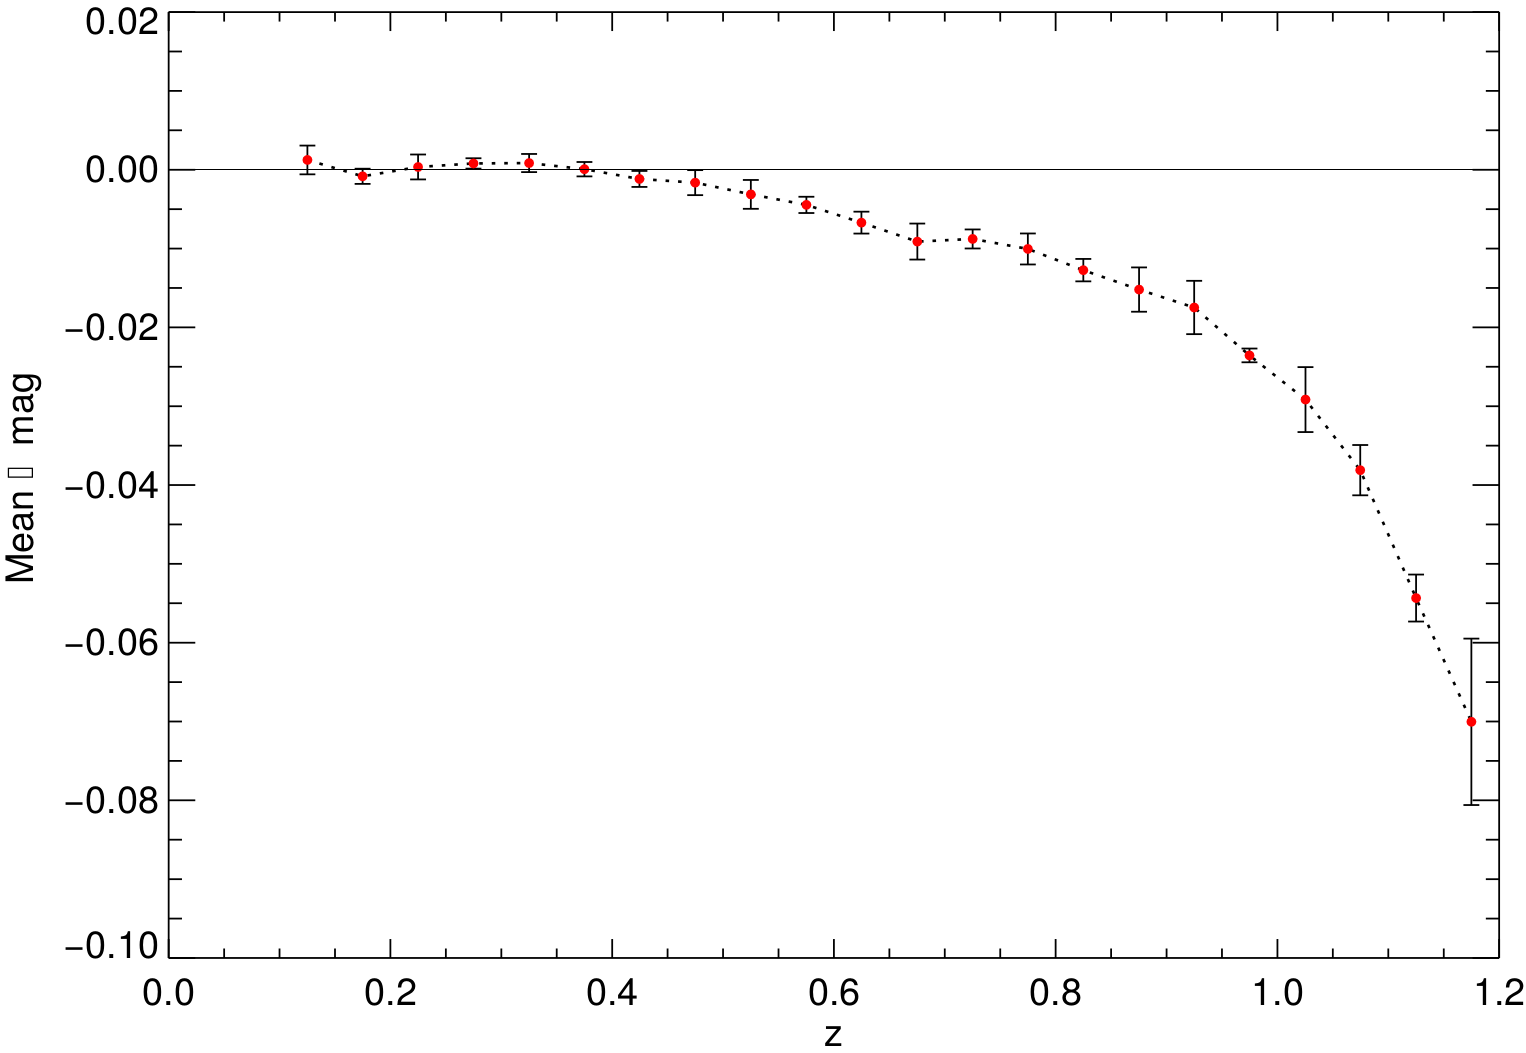
\includegraphics[width=.5\linewidth]{snls_malmquist.png}
    % \captionsetup{justification=centering}
    \caption[Biais de \textsc{Malmquist} moyen en fonction du redshift pour le
    sondage SNLS]{Biais de \textsc{Malmquist} et de sélection spectroscopique
        moyen en fonction du redshift pour le sondage SNLS d'après des
        simulations.\smallbreak Figure de~\cite{perrett2010}.}
    \label{fig:snlsmalm}
\end{SCfigure}

\paragraph*{De la même manière pour PS1} leurs SNe~Ia sont entre $0,2 < z <
0,4$~; la profondeur à 5$\sigma$ dans la bande $g$ est de \SI{23,1}{mag} d'après
\cite{rest2014} et mène à $z_{\lim}=0,31$, en correspondance avec la Figure~6
de~\cite{scolnic2018} par exemple, recopiée Figure~\ref{fig:ps1malm}. De manière
conservative, cette figure suggère une limite plus prononcée à $z_{\lim}=0,27$~;
ces deux valeurs constituent donc les redshifts limites de PS1 pour la partie
fiducielle et conservative, respectivement, de notre échantillon.

\begin{SCfigure}[0.7][ht!]
    \centering
    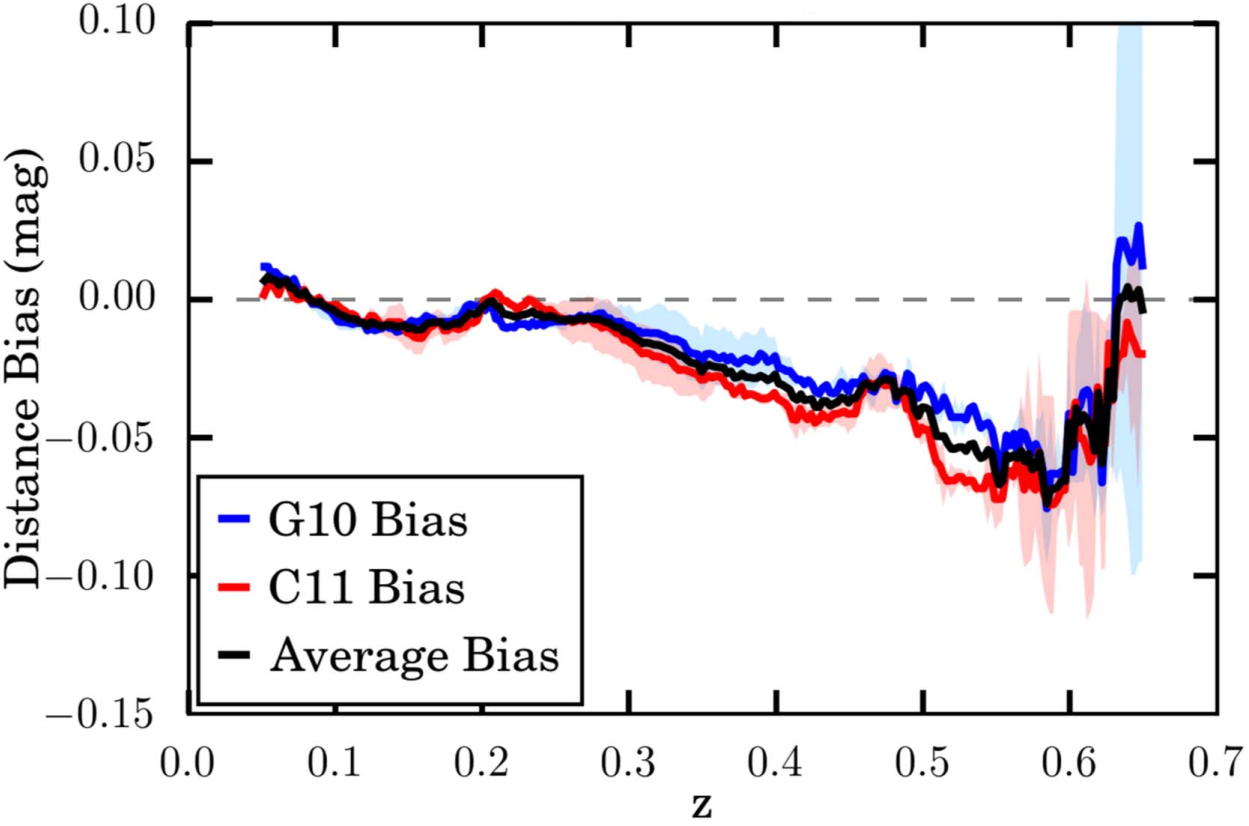
\includegraphics[width=.5\linewidth]{ps1_malmquist.png}
    % \captionsetup{justification=centering}
    \caption[Biais de \textsc{Malmquist} moyen en fonction du redshift pour le
    sondage PS1]{Biais de \textsc{Malmquist} moyen dû aux effets de sélection
        en fonction du redshift pour le sondage PS1, d'après des simulations et
        pour deux modèles de dispersion intrinsèques différents et leur moyenne.
        \smallbreak Figure de~\cite{scolnic2018}.}
    \label{fig:ps1malm}
\end{SCfigure}

\paragraph*{Dans le même intervalle pour SDSS} la magnitude limite est de
\SI{22,5}{mag} d'après~\cite{dilday2008} et~\cite{sako2008}~; cette valeur 
impliquerait $z_{\lim}=0,24$, mais les sondages SDSS se sont confrontés à une
limitation dans leurs capacités spectroscopiques. Comme indiqué
dans~\cite{kessler2009a} Section~2, les données de la première année de SDSS ont
favorisé les SNe~Ia de magnitude $r < \SI{20,5}{mag}$ pour identification
spectroscopique, ce qui correspondrait à une coupe de redshift à 0,15. Le reste
du programme a bénéficié de meilleures ressources spectroscopiques
et~\cite{kessler2009a} et~\cite{dilday2008} font preuve d'une complétude
raisonnable jusqu'à $z=0,2$. La Figure~3 de~\cite{conley2011}, montrée
Figure~\ref{fig:sdssmalm} et donnant l'évolution du biais de \textsc{Malmquist}
en fonction du redshift confirme ces hypothèses. En nous basant sur ces faits,
nous avons choisi $z_{\lim}=0,20$ et $z_{\lim}=0,15$ pour nos échantillons
fiduciel et conservatif respectivement.

\begin{SCfigure}[0.7][ht!]
    \centering
    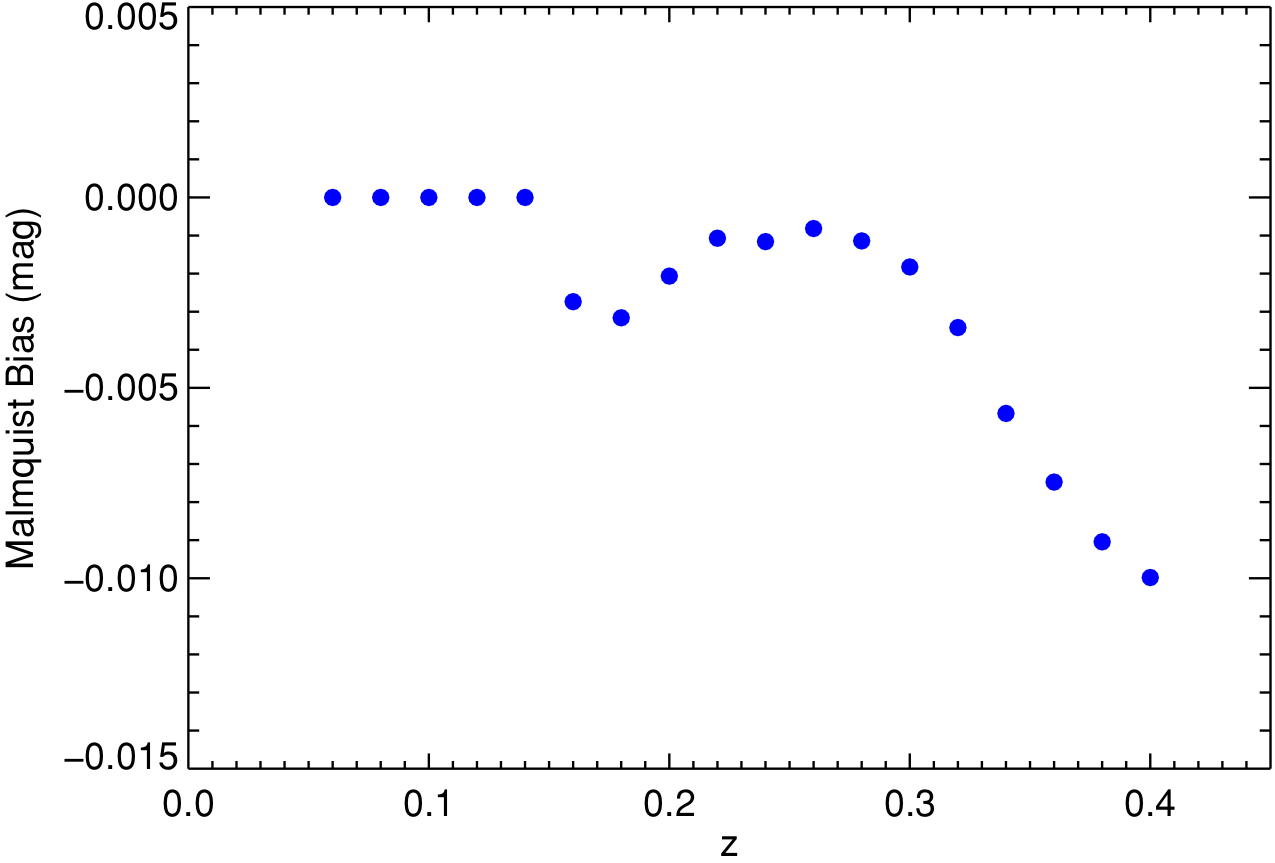
\includegraphics[width=.5\linewidth]{sdss_malmquist.png}
    % \captionsetup{justification=centering}
    \caption[Biais de \textsc{Malmquist} moyen en fonction du redshift pour le
    sondage SDSS]{Biais de \textsc{Malmquist} moyen en fonction du redshift
        pour le sondage SDSS. La forte baisse à $z=0,15$ est un artéfact dû à la
        discontinuité du modèle d'efficacité spectroscopique et n'a que peu
        d'effet sur les contraintes cosmologiques.\smallbreak Figure
    de~\cite{conley2011}.}
    \label{fig:sdssmalm}
\end{SCfigure}

Cette approche est totalement systématique et reproductible, et donne des
$z_{\lim}$ similaires à l'approche statistique~; cette observation conforte donc
les résultats et choix de magnitudes limites, et ce sont ces résultats
analytiques que nous avons conservés dans notre étude. La comparaison des
limites par les deux méthodes et le nombre de données conservées avec les
limites analytiques dans les cas fiduciels et conservatifs sont indiqués
Table~\ref{tab:zlimsample}.

\begin{table}[ht]
    \centering
        \caption{Composition en SNe~Ia de notre échantillon.}
        \label{tab:zlimsample}
    \begin{threeparttable}
        \makebox[\linewidth]{%
        \begin{tabular}{lccc}
            \toprule
            \multirow{2}[2]{*}{Sondage} &
            \multicolumn{2}{c}{$z_{\lim}$} &
            \multirow{2}[2]{*}{$N_{\rm SN}$}\\
            \cmidrule(lr){2-3}
            & Statistique & Analytique & \\
            \midrule
            SNf &
            \multicolumn{2}{c}{0,08} &
            114 \\
            SDSS & 
            0,204$^{+0,001}_{-0,001}$ & 0,20 (0,15) &
            167 (82) \\
            PS1 &
            0,284$^{+0,006}_{-0,008}$ & 0,31 (0,27) &
            160 (122) \\
            SNLS &
            0,615$^{+0,003}_{-0,003}$ & 0,60 (0,55) &
            102 (78) \\
            HST &
            \multicolumn{2}{c}{--} &
            26 \\
            \midrule
            Total & \multicolumn{2}{c}{--} &
            569 (422)\\
            \bottomrule
    \end{tabular}}
        \begin{tablenotes}[flushleft]
        \item\small \textbf{\hspace{-3,2pt}Notes.} L'échantillon et notamment le
            nombre de SNe utilisées suivent les limites analytiques. Les nombres
            entre parenthèses correspondent aux limites conservatives.
        \end{tablenotes}
    \end{threeparttable}
\end{table}

\subsection{Présentation}\label{ssec:dataset}

Par rapport aux analyses cosmologiques générales, notre étude impose une forte
sélection sur des données déjà soigneusement choisies~: seulement 43\% (SNLS) à
57\% (PS1) de SNe~Ia sont conservées. Les distributions en redshift des 3
sondages coupés sont présentées Figure~\ref{fig:cuts}. Nous y observons que les
limites sont globalement situées avant le pic de ces histogrammes, suivant la
logique guidant cette chute (cf. Section~\ref{sec:compl}) et confortant
également les analyses qui y ont mené. Cette hypothèse est testée
Section~\ref{ssec:testvl}.

\begin{figure}
    \centering
    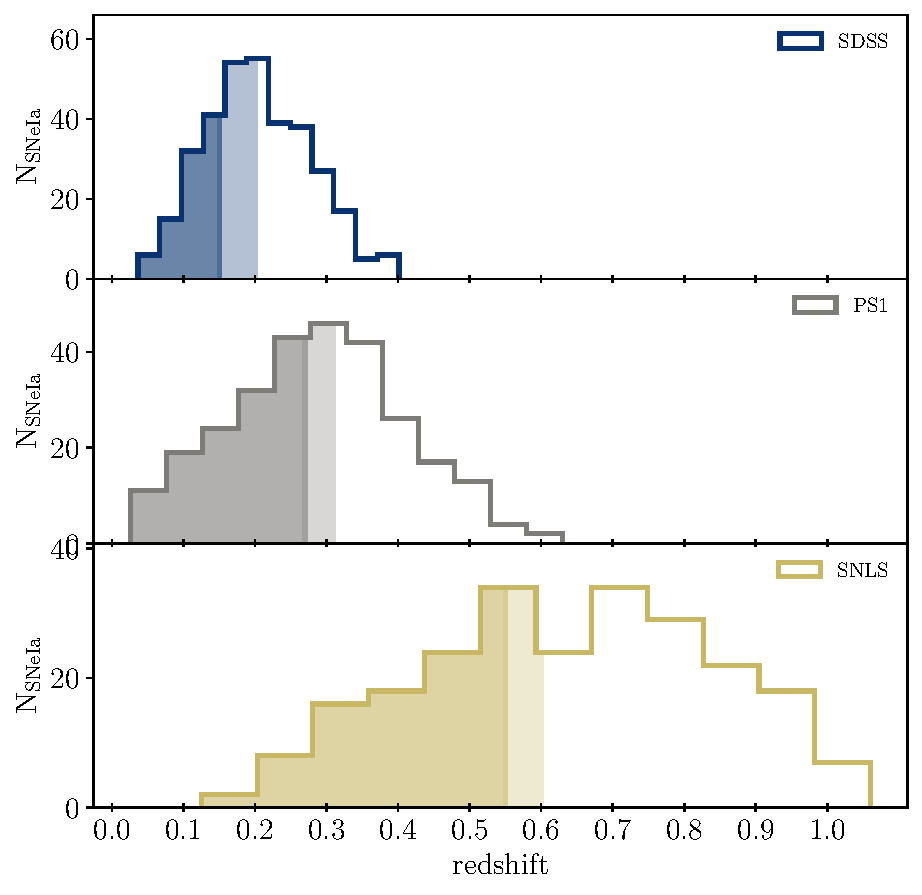
\includegraphics[width=0.80\linewidth]{hist_surveys_cuts_nospace}
    \caption[Histogrammes des sondages coupés pour notre étude]{\textit{De haut
        en bas}: Histogrammes en redshift des SNe~Ia des sondages SDSS, PS1 et
        SNLS \citep[données de Pantheon,][]{scolnic2018}. Les parties colorées
        représentent les distributions de SNe~Ia conservées dans notre analyse,
        considérées exemptes d'effets de sélection observationnels (cf.
        Section~\ref{sssec:maglim}). Les couleurs foncées (claires) représentent
        les limites conservatives (fiducielles) de nos coupes de sélection
    indiquées dans la Table~\ref{tab:zlimsample}.}
    \label{fig:cuts}
\end{figure}

En combinant les 5 sondages de notre analyse, nous pouvons tracer leur
distribution d'étirement en fonction du redshift. Nous en présentons un
graphique ainsi que l'histogramme complet Figure~\ref{fig:sample}. En supposant
l'échantillon affranchi d'effets de sélection, nous pouvons lire sur ce
graphique une première idée de l'évolution en redshift que nous supposons issue
du changement des propriétés moyennes des SNe~Ia avec l'âge de leur
environnement. En effet, nous observons que la fraction de SNe~Ia présentant un
faible étirement, typiquement $x_1 < -1$, semble décroître avec le redshift alors
que la population d'étirement $> 1$ semble toujours peuplée~; à noter qu'ici le
redshift est en échelle logarithmique, expliquant le tassement horizontal.
Quantitativement, les SNe~Ia à haut redshift présentent un plus grand étirement
moyen ($0,34 \pm 0,10$ à $z \approx 0,65$) que celles à bas redshift ($-0,17 \pm
0,10$ à $z \approx 0,05$). Cette idée est confirmée dans le chapitre suivant,
Section~\ref{sec:xres}.

\begin{figure}
    \centering
    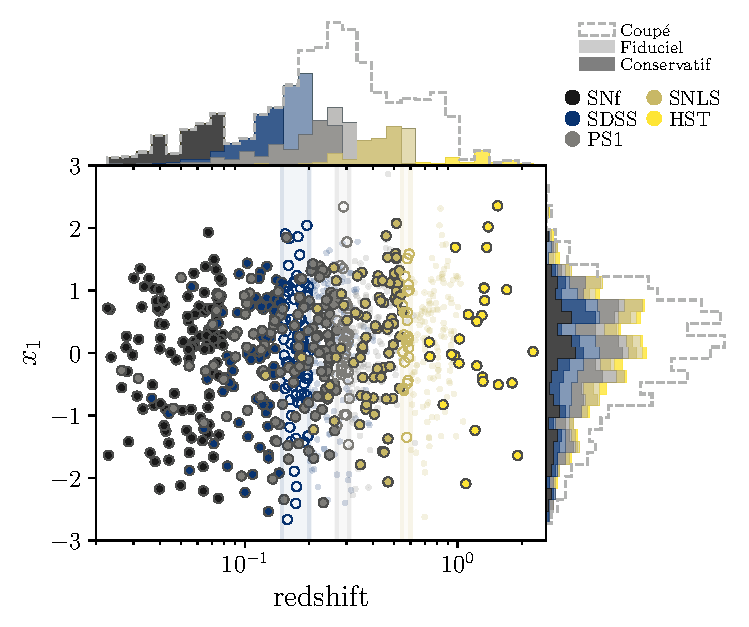
\includegraphics[width=0.95\linewidth]{stretchs-cut_btw_sup_hist_stac_x1}
    \caption[Présentation des données d'étirement en fonction du redshift pour
    l'échantillon complet]{\textit{En bas}~: étirement des courbes de lumière
        ajustées avec \textsc{\texttt{SALT2.4}} en fonction du redshift en
        échelle logarithmique pour chaque sondage de cette analyse (cf.\
        légende). Les points pleins, creux et transparents correspondent aux
        échantillons conservatif, fiduciel et total, respectivement. \textit{En
        haut}~: histogrammes en redshift superposés, en sombre, clair et
        pointillé pour les échantillons conservatif, fiduciel et total,
        respectivement (cf.\ légende). \textit{À droite}~: histogrammes en
        étirement superposés. Notre hypothèse de travail se base sur le
        dépeuplement des étirements $< -1$ avec le redshift, que nous pouvons
        apercevoir dans les histogrammes de droite~: relativement aux données
    $x_1 > -1$, cette partie se peuple moins.}\label{fig:sample}
\end{figure}

\subsection{Confirmation d'hypothèse}\label{ssec:testvl}

% Dans la Section précédente, nous avons construit des échantillons limités en
% volume à partir d'ensembles limités en magnitude par le biais de simples coupes
% en redshift. Cette approche simplifiée est statistiquement sous-optimale, mais
% devrait suffire pour éprouver notre hypothèse concernant la compatibilité de
% l'évolution de l'étirement avec le redshift avec le modèle de \cite{rigault2020}.
% Cependant, il reste possible qu'une fonction complexe d'effets de sélection
% observationnels liée aux efficacités de suivi spectroscopique en-deçà de nos
% limites (fiducielles voire conservatives) affecte notre échantillon, le rendant
% de fait pas totalement limité en volume~; ceci biaiserait alors notre conclusion
% quant à l'existence d'une évolution astrophysique de la population des SNe~Ia.
% 
% Pour tester l'existence de biais de sélection observationnels résiduels dans
% notre échantillon, nous avons comparé 

Dans la Section précédente, nous avons construit des échantillons limités en
volume à partir d'un ensemble d'échantillons limités en magnitude en utilisant
des coupures simples de redshift. Cette approche simplifiée est
statistiquement sous-optimale, mais devrait suffire pour tester notre question
clé, à savoir si l'évolution de l'étirement avec le redshift est compatible avec le
modèle de \cite{rigault2020}. Cependant, il reste possible qu'une fonction de
sélection observationnelle complexe liée aux efficacités de suivi
spectroscopique en deçà de nos coupures fiducielles (voire conservatives) puisse
encore affecter notre échantillon, le rendant non entièrement limité en volume~;
cela fausserait alors notre conclusion sur la dérive astrophysique de la
population SNe Ia.

Pour tester l'existence d'éventuels biais de sélection observationnels dans
notre échantillon, nous avons comparé les distributions d'étirement et de couleur
des SNe~Ia provenant de différents ensembles de données dont les plages de
redshifts se chevauchent~: ces distributions devraient être similaires si elles
reflètent la même population mère sous-jacente. Nous notons que la plage de
redshift doit être suffisamment étroite pour que toute dérive soit négligeable.

Les deux échantillons qui se chevauchent le plus en termes de redshift sont PS1
et SDSS dans la plage de redshift $0,10 < z < 0,20$ (voir
Figure~\ref{fig:sample}). Ce sous-échantillon est constitué des 146 SNe~Ia à
l'extrémité haute des redshifts de SDSS et est donc le plus susceptible d'être
affecté par des effets de sélection observationnels résiduels (voir la
discussion correspondante dans la Section~\ref{ssec:malm}). Sur cette même plage
de redshift, PS1 compte 52 SNe~Ia qui se trouvent dans les tranches de redshift
les plus basses et qui sont donc peu susceptibles d'être affectées par un
problème de sélection observationnelle. Afin d'identifier les incohérences
potentielles entre les sous-échantillons PS1 et SDSS, la Figure~\ref{fig:testvl}
(panneaux supérieurs) compare la distribution des étirements et des couleurs de
ces deux études. Les valeurs $p$ du test de similarité de
\textsc{Kolmogorov-Smirnov} (KS) qui en résultent ($p > 10\%$) n'indiquent
aucune raison de croire que les deux distributions ne sont pas issues d'une même
population sous-jacente, ce qui aurait été le cas si l'une ou l'autre des
distributions était affectée par des effets de sélections, en accord avec
l'impression visuelle de la Figure~\ref{fig:testvl}.

\begin{figure}[ht]
    \centering
    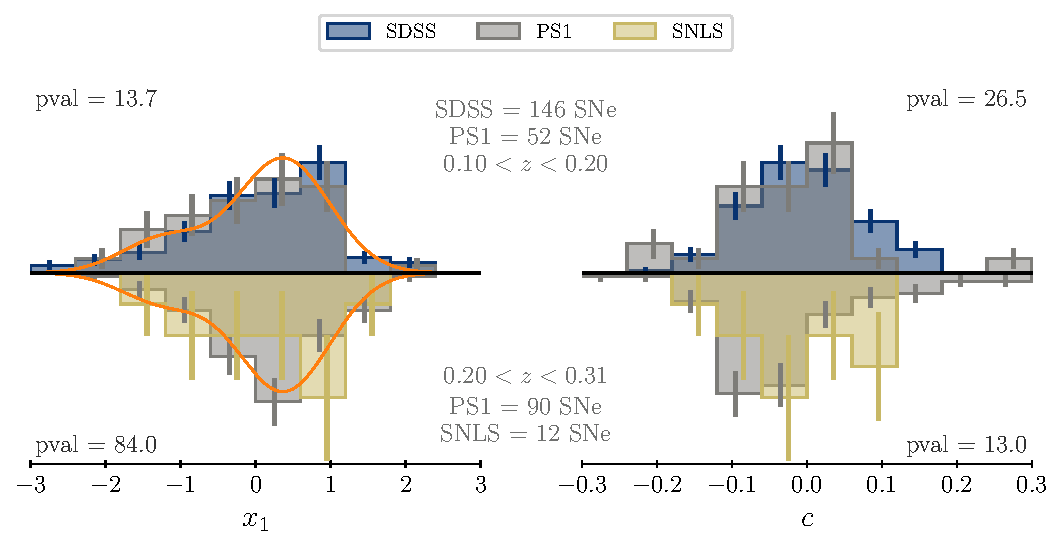
\includegraphics[width=.8\linewidth]{both-cut_SDSS_SNLS_PS1}
    % \captionsetup{justification=centering}
    \caption[Histogrammes de test de similarité de \textsc{Kolmogorov-Smirnov}
    entre les sondages SDSS et PS1 d'une part, PS1 et SNLS d'autre part, en
    étirement et en couleur]{Histogrammes de distribution d'étirement (gauche) et
        de couleur (droite) de différents relevés se chevauchant en redshift.
        \textit{Vers le haut}~: SDSS et PS1 dans la plage de redshift $0,10 < z
        < 0,20$. \textit{Vers le bas}~: PS1 et SNLS dans la gamme de redshift
        $0,20 < z < 0,31$. Les barres d'erreur représentent le bruit de Poisson.
        Notre modèle d'évolution en redshift (défini plus loin,
        Section~\ref{ch:stretch}) est illustré en orange à la valeur moyenne des
        plages de redshifts, 0,15 et 0,25 respectivement. Les valeurs $p$ du
        test de \textsc{Kolmogorov-Smirnov} sont indiquées en haut (en bas) de
        chaque panneau et ne montrent aucun signe que les distributions
        d'étirement et de couleur de SDSS et PS1 (PS1 et SNLS) ne sont pas
    tirées des mêmes distributions sous-jacentes.}
    \label{fig:testvl}
\end{figure}

Nous avons effectué une analyse similaire pour PS1 et SNLS sur la plage de
redshift $0,20 < z < 0,31$ (Figure~\ref{fig:testvl}, panneaux inférieurs), où la
même conclusion peut être tirée~: il n'y a pas de signe significatif de
divergence dans les distributions d'étirement et de couleur entre les extrémités
basse et haute de nos échantillons fiduciels de SNLS et PS1, respectivement.
Néanmoins, la petite taille de l'ensemble de données SNLS à $z < 0,31$ (12
SNe~Ia contre 90 pour PS1) limite la sensibilité de ce test, et seule une forte
déviation serait perceptible. L'extension de la plage de redshift à $0,20 < z <
0,40$ (bien que nous n'ayons pas de données PS1 au-dessus de 0,3) permet
d'augmenter le sous-échantillon SNLS à 31, mais la valeur $p$ de l'étirement
reste élevée (34\%).

Nous soulignons enfin que la couleur des SNe~Ia est plus sujette aux effets de
sélection observationnelle que l'étirement, comme l'illustre la
Figure~\ref{fig:maglim}~; voir également la Figure~3 de~\cite{kessler2017}, par
exemple. Par conséquent, comme la comparaison des distributions de couleurs ne
montre aucune indication significative d'un effet de sélection observationnelle
résiduel, cela renforce notre affirmation selon laquelle nos critères de
sélection simples basés sur le redshift sont suffisants pour construire les
échantillons complets de SNe~Ia nécessaires pour tester l'évolution du redshift
de la distribution d'étirement.

\section{Application à ZTF}\label{sec:ztfsam}
Au moment de rédiger cette thèse, la deuxième publication de données de ZTF est
en cours. Ainsi, bien qu'il ne fasse pas partie de cette étude de manière
stable, nous nous intéressons à son intégration dans notre travail. C'est
pourquoi nous présentons ici notre confection de la partie limitée de ZTF.

\subsection{Redshift limite}\label{ssec:ztflim}
%\appssec{Redshift limite}{ssec:ztflim}

\paragraph*{Sa magnitude limite} est donnée à
\SI{20.4}{mag}\footnote{\href{https://www.ztf.caltech.edu/ztf-camera.html}
{https://www.ztf.caltech.edu/ztf-camera.html}}, ce qui se convertirait à un
$z_{\lim} = 0,11$, mais la SEDm est indiquée avoir une classification correcte
entre $[18,5-19]$\si{mag} \citep{fremling2020}, ce qui implique des limites
$z_{\lim} = [0,044-0,055]$ respectivement. Ces résultats sont confortés par une
étude du sondage effectuée par \textsc{Amenouche} et al. (\textit{en
préparation}), utilisant le module Python
\texttt{simsurvey}
\footnote{\href{https://github.com/ZwickyTransientFacility/simsurvey}
{https://github.com/ZwickyTransientFacility/simsurvey}} de ZTF
\citep{feindt2019}. Initialement utilisé pour permettre le pronostic des
résultats du sondage, l'utilisation de journaux d'observation réels indique que
l'échantillon devrait être limité en volume jusqu'à $z \approx 0,06$. Ainsi, ce
sont les valeurs $z_{\lim} = 0,044$ et $z_{\lim} = 0,055$ qui constituent nos
limites conservative et fiducielle pour ZTF, respectivement. Le
Tableau~\ref{tab:zlimztf} résume les informations de coupe pour ZTF.

\begin{table}[ht]
    \centering
        \caption{Composition en SNe~Ia pour notre échantillon ZTF.}
        \label{tab:zlimztf}
    \begin{threeparttable}
        \makebox[\linewidth]{%
        \begin{tabular}{lcc}
            \toprule
            Sondage & $z_{\lim}$ & $N_{\rm SN}$\\
            \midrule
            ZTF & 0,055 (0,044) & 638 (393) \\
            \midrule
            Total & -- & 1379 (987)\\
            \bottomrule
    \end{tabular}}
        \begin{tablenotes}[flushleft]
            \item\small \textbf{\hspace{-3,2pt}Notes.} Le nombre total inclus les
                données de la section précédente.
        \end{tablenotes}
    \end{threeparttable}
\end{table}

\subsection{Présentation}\label{ssec:ztfpres}
%\appssec{Présentation}{ssec:ztfpres}

Dans le cas de ZTF, la coupe en redshift est encore plus sévère que pour les
autres sondages~; c'est en effet 28\% des données qui sont conservées. Il reste
cependant que sa partie fiducielle est à elle seule plus peuplée que la totalité
de notre échantillon de base. L'inclusion de ces données augmentera donc la
statistique et la robustesse de notre étude d'un facteur non-négligeable. La
Figure~\ref{fig:ztfsample} en montre la distribution des données d'étirement en
fonction du redshift.

\begin{figure}[ht!]
    \centering
    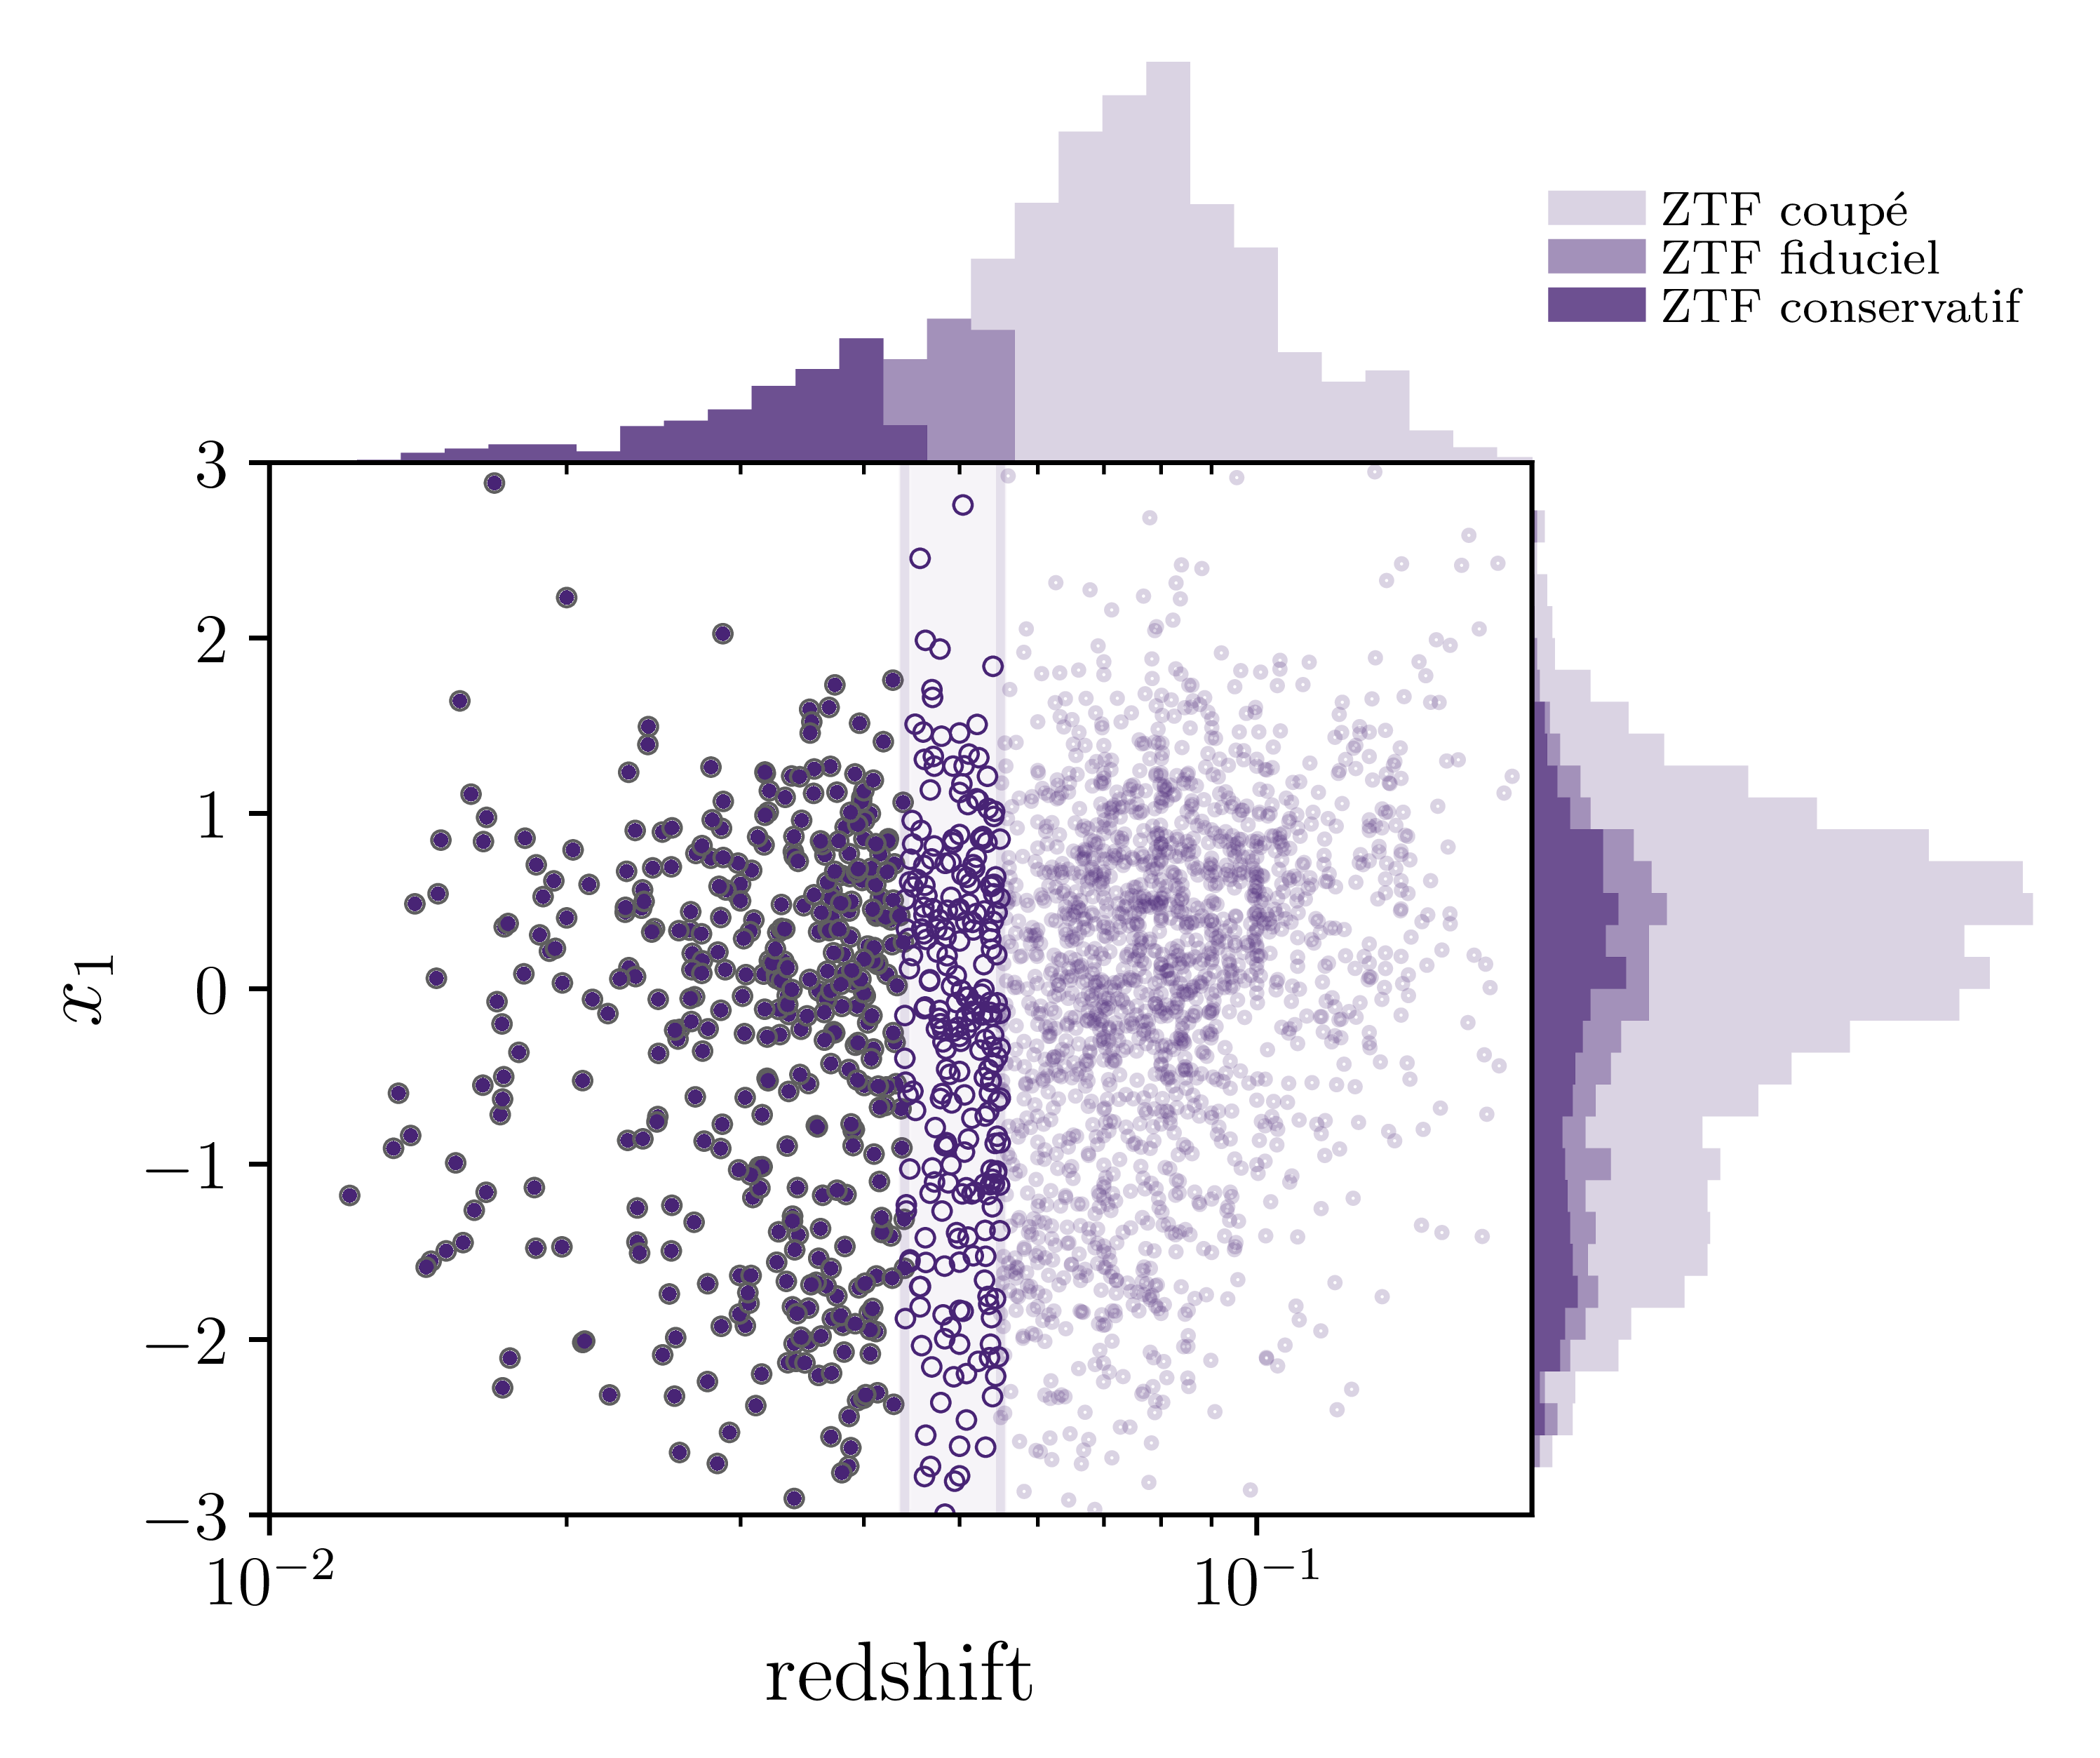
\includegraphics[width=0.80\linewidth]{stretchs-cut_btw_sup_hist_ztf_x1}
    \caption[Présentation des données d'étirement en fonction du redshift pour
    ZTF]{\textit{En bas}~: étirement des courbes de lumière ajustées avec
        \textsc{\texttt{SALT2.4}} en fonction du redshift en échelle
        logarithmique pour ZTF (cf.~légende). Les points pleins, creux et
        transparents correspondent aux parties conservative, fiducielle et
        totale respectivement. \textit{En haut}~: histogrammes en redshift
        superposés, en sombre, clair et très clair pour les parties
        conservative, fiducielle et totale respectivement (cf.\ légende).
        \textit{À droite}~: histogrammes en étirements superposés, même
    légende.}\label{fig:ztfsample}
\end{figure}

Sur cette figure, nous pouvons d'ores et déjà observer la présence d'un sursaut
à basse valeur dans la distribution des étirements ($x_1 \approx -1.5$). Sa
présence est en accord avec l'étude de la distribution d'étirement du chapitre
suivant. Ces données étant arrivées après l'étude en question, sa présence en
conforte les résultats~; nous en discutons Section~\ref{sec:xztf}.

Au sein de ce sondage, la dérive de l'âge avec le redshift est considérée comme
négligeable d'après l'Équation~\refeq{eq:deltaz} dont l'évolution est montrée
Figure~\ref{fig:deltaz}. Pour voir une éventuelle variation de la population à
petit étirement avec le redshift, nous présentons Figure~\ref{fig:zsample}
l'échantillon de base combiné aux données de ZTF. La présence de nombreuses
données à $z \lesssim 0,05$ dû à ZTF écrase les données des autres échantillons
s'étalant jusqu'à $z = 2.26$ pour la représentation logarithmique, mais permet
une meilleure visualisation de la potentielle évolution de l'étirement avec le
redshift grâce aux histogrammes de la partie droite.

\vfill
\begin{figure}[ht!]
    \centerfloat
    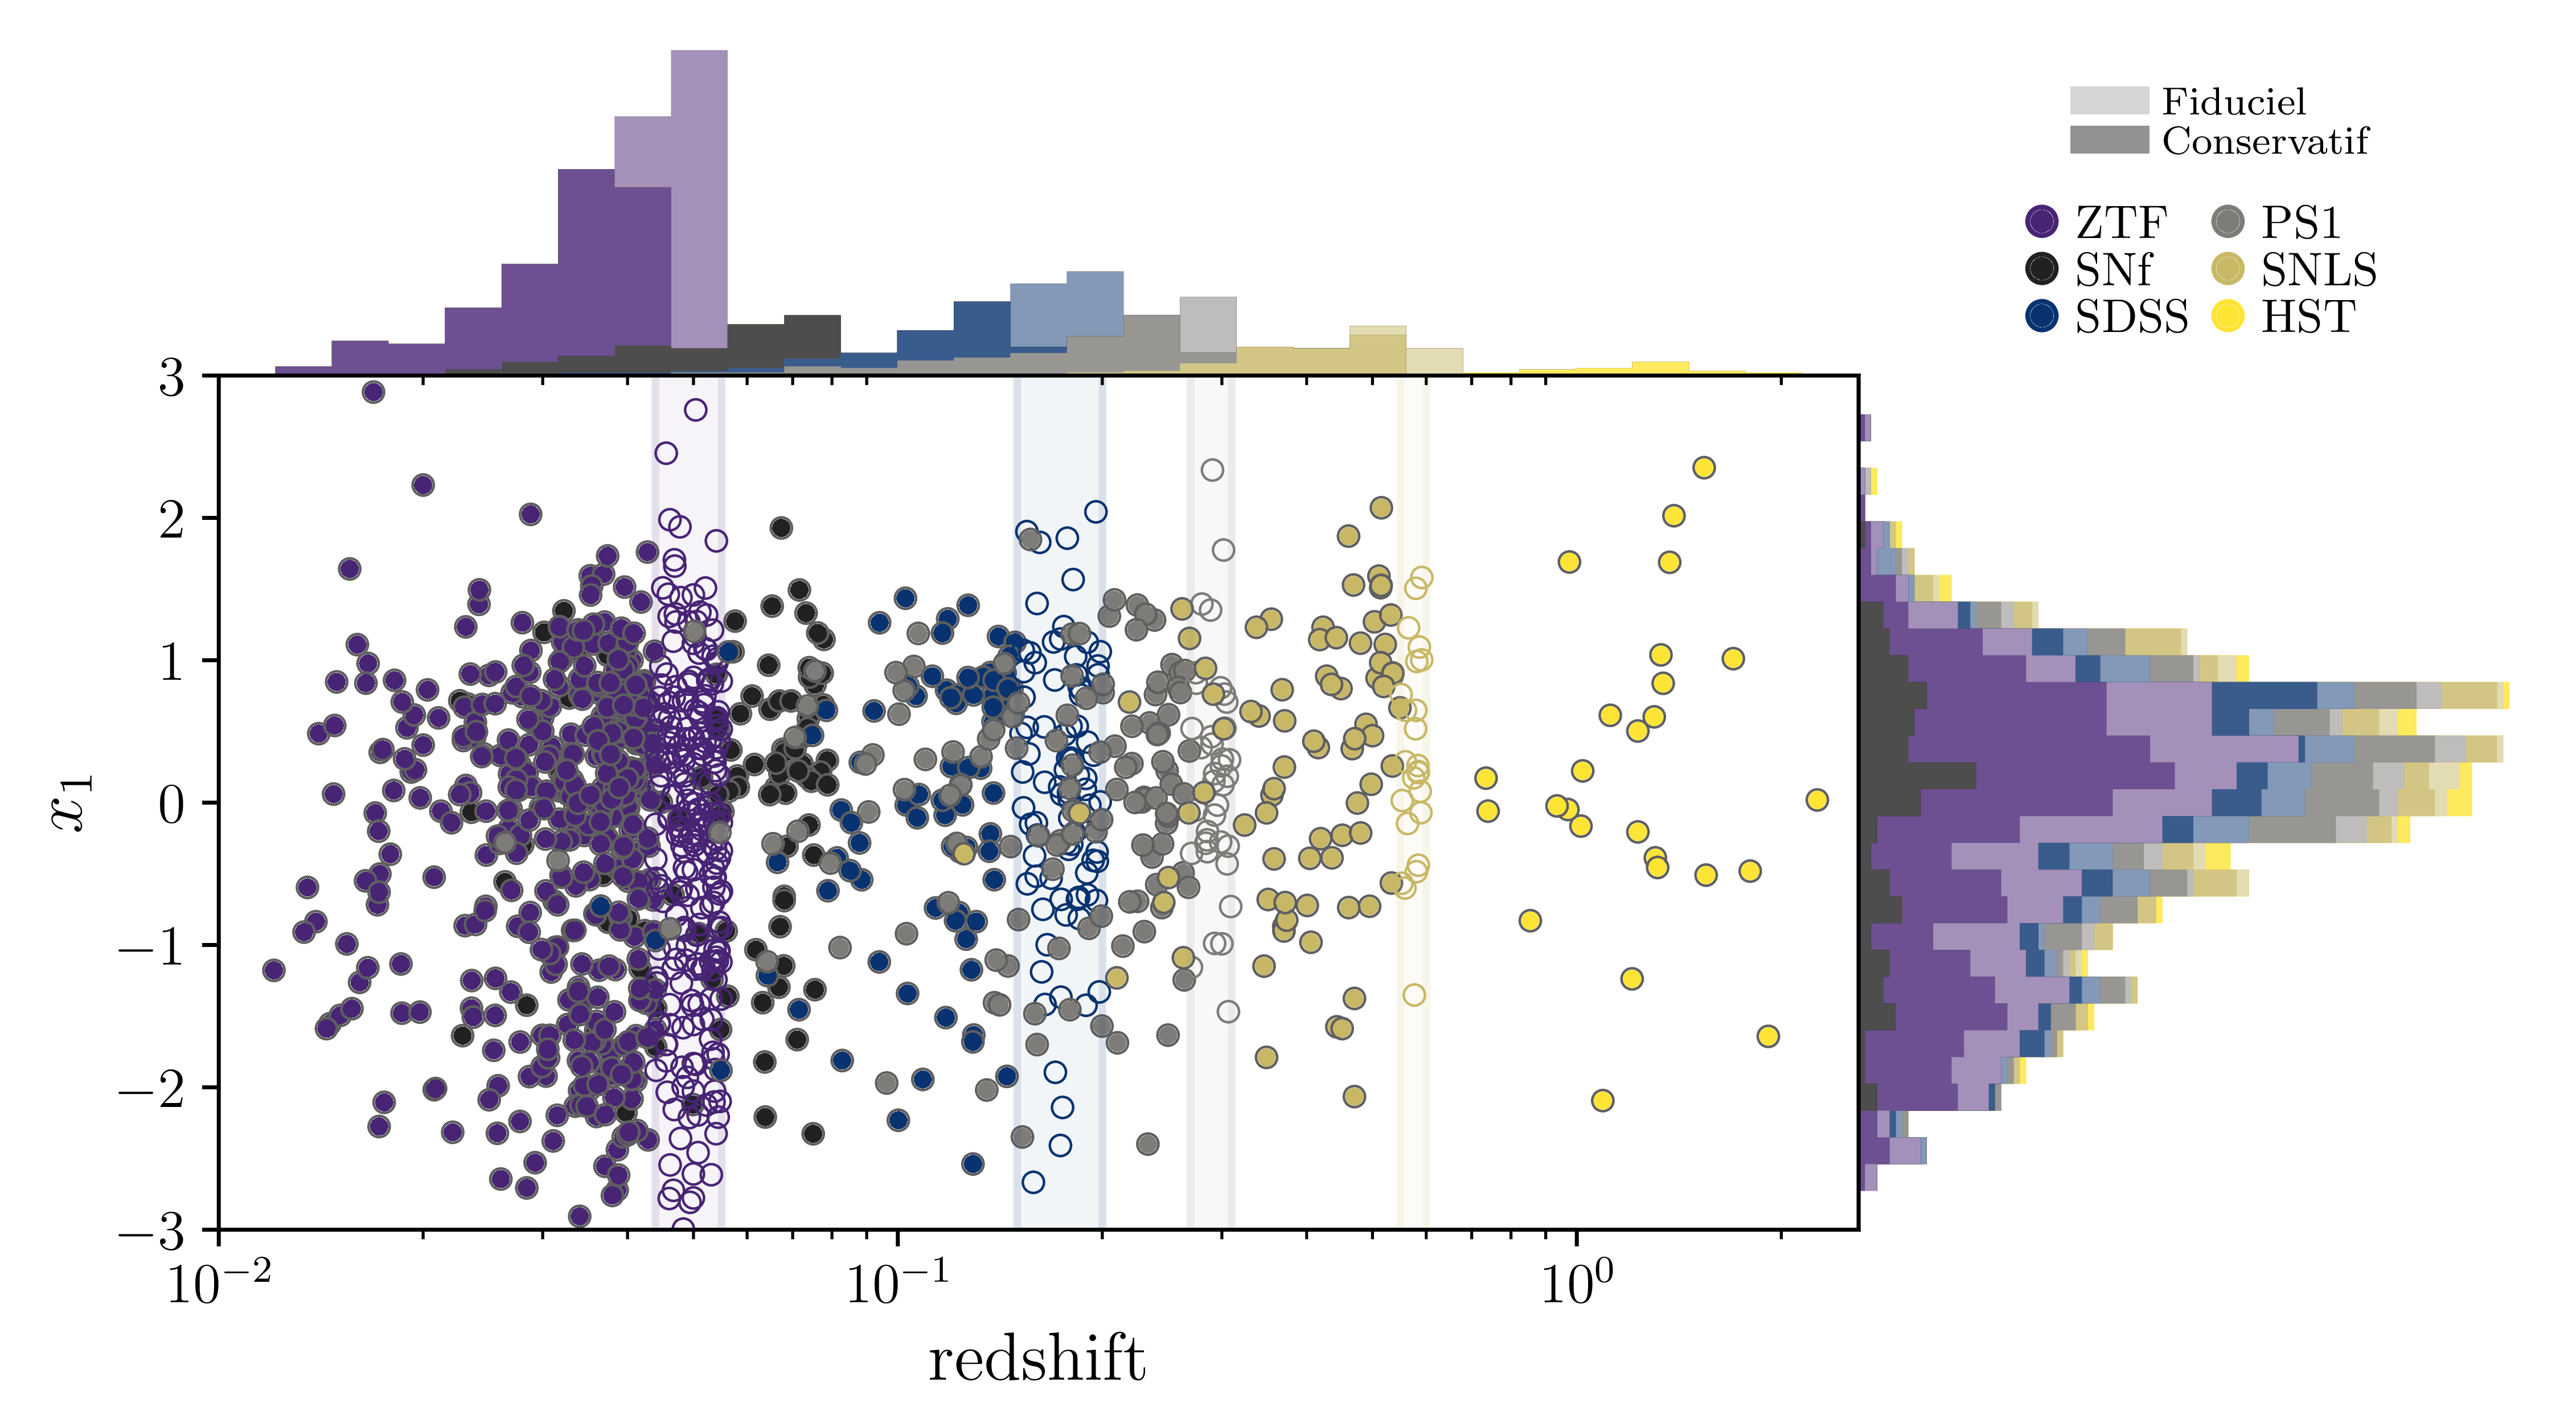
\includegraphics[width=1.1\linewidth]{stretchs-cut_btw_hist_stac_ztf_x1}
    \caption[Présentation des données d'étirement en fonction du redshift pour
    l'échantillon de base combiné aux données de ZTF]{\textit{En bas}~:
        étirement des courbes de lumière ajustées avec \textsc{\texttt{SALT2.4}}
        en fonction du redshift en échelle logarithmique pour l'intégrité des
        sondages apparaissant dans l'étude de la dérive de l'étirement avec le
        redshift (cf.~légende). Les points pleins et creux  correspondent aux
        parties conservative et fiducielle  respectivement. \textit{En haut}~:
        histogrammes en redshift superposés, en sombre et clair pour les parties
        conservative et fiducielle respectivement (cf.\ légende). \textit{À
        droite}~: histogrammes en étirements superposés, même
    légende.}\label{fig:zsample}
\end{figure}
\vfill

\clearpage

\thispagestyle{plain}
\vfill
\minilof
\vfill
\minilot
\vfill

% \bibliographystyle{../main/aa_url}
% \shorthandoff{:}
% \bibliography{../chapters/99_references}

\end{document}
